\documentclass[11pt,a4paper]{article}
\usepackage[margin=2.1cm]{geometry}
\usepackage{fontspec}
\setmainfont{Bitstream Charter}
\setsansfont{DejaVu Sans}[Scale=0.9]
\setmonofont{DejaVu Sans Mono}[Scale=0.82]
\usepackage{microtype}
\usepackage{graphicx}
\usepackage{booktabs}
\usepackage{caption}
\usepackage{subcaption}
\usepackage{float}
\usepackage{xcolor}
\usepackage[hidelinks]{hyperref}
\usepackage{titlesec}
\captionsetup{font=small,labelfont=bf}
\titleformat{\section}{\large\bfseries}{\thesection.}{0.5em}{}
\titlespacing*{\section}{0pt}{1.0ex}{0.5ex}
\titleformat{\subsection}{\normalsize\bfseries}{}{0em}{}
\titlespacing*{\subsection}{0pt}{0.8ex}{0.3ex}
\setlength{\parskip}{0.45ex}
\setlength{\parindent}{0pt}
\graphicspath{{../figures/}}

\begin{document}

\begin{center}
{\LARGE\bfseries Understanding Student Performance in Secondary-School Mathematics}\\[0.6ex]
{\large Final Project, Scenario 2 \;|\; Data Analytics and Statistics with Applications (LEAP)}\\[0.4ex]
Tarık Beyhan \;|\; October 2026
\end{center}

\noindent\textbf{Research question.} Which student background and behavioural characteristics explain final Mathematics performance, what drives the risk of failing, and what are the realistic limits of these observational data?

\noindent\textbf{Summary.} Across both linear and logistic specifications, past academic failure is the single strongest predictor of poor final performance and course failure. Higher maternal education correlates with better outcomes, while frequent socialising is linked to lower marks. Still, the models capture only under a fifth of the total variance in grades. Importantly, the 38 students recorded with a grade of zero appear to be non-attendees or dropouts rather than test-takers who earned zero; handling them separately significantly shifts several estimates, particularly the effect of absences. Given the cross-sectional, observational structure, these results indicate correlations rather than direct interventions.

%==============================================================================
\section{Data preparation and screening}

The analysis uses the Mathematics subset of the UCI Student Performance dataset (Cortez, 2008), comprising 395 students across two Portuguese secondary schools: Gabriel Pereira (349) and Mousinho da Silveira (46). The target outcome is the final grade, \texttt{G3}, evaluated on a 0--20 scale, alongside a binary pass indicator ($\texttt{G3} \geq 10$). Following the project brief, earlier term marks (\texttt{G1} and \texttt{G2}) were excluded from the predictor pool to focus on broader student background and behaviour.

Categorical survey items with natural ordering (such as parental education levels from 0 to 4, study time, and self-reported health or social habits on 1--5 scales) were retained as numeric integers for baseline modelling, while purely nominal fields were set as factors in R. 

The dataset contains no missing cells, but inspection revealed an anomaly: 38 students (9.6\%) have a final grade of exactly 0, with a complete void between 1 and 3. All 38 have zero recorded absences (compared to 22\% zero-absence rates across the rest of the cohort), and their mean first-period grade was 7.5. This pattern suggests administrative dropouts or exam absentees whose attendance tracking simply ceased, rather than students who sat the exam and scored zero. Because abandoning the course still constitutes failing in practice, I retain them in the main models but evaluate the stability of the conclusions via a sensitivity check without them.

From an ethics standpoint, while individual names are omitted, the survey touches on sensitive areas including home stability, substance use, and personal relationships. Because the smaller school has only 46 records, cross-referencing demographic variables could lead to re-identification. The findings are intended to highlight broad patterns where academic assistance might help, not to profile or categorise individuals.

%==============================================================================
\section{Exploratory data analysis}

The average final grade is 10.4 with a standard deviation of 4.6 (median 11, IQR 8--14). Excluding the cluster at zero, the distribution is roughly bell-shaped around 11 (Figure~\ref{fig:dist}). Overall, 67.1\% of the cohort passed (265 students) and 32.9\% failed (130 students), with the 38 zero-grade cases accounting for nearly thirty percent of all failures. Absences show marked right-skew (mean 5.7, median 4, reaching up to 75). Most participants had zero previous course failures (312 students), whereas 50 had one, 17 had two, and 16 had three or more. The gender split is fairly even (208 female, 187 male), whereas ambition for higher education is heavily skewed towards ``yes'' (375 vs 20).

\begin{figure}[H]
\centering
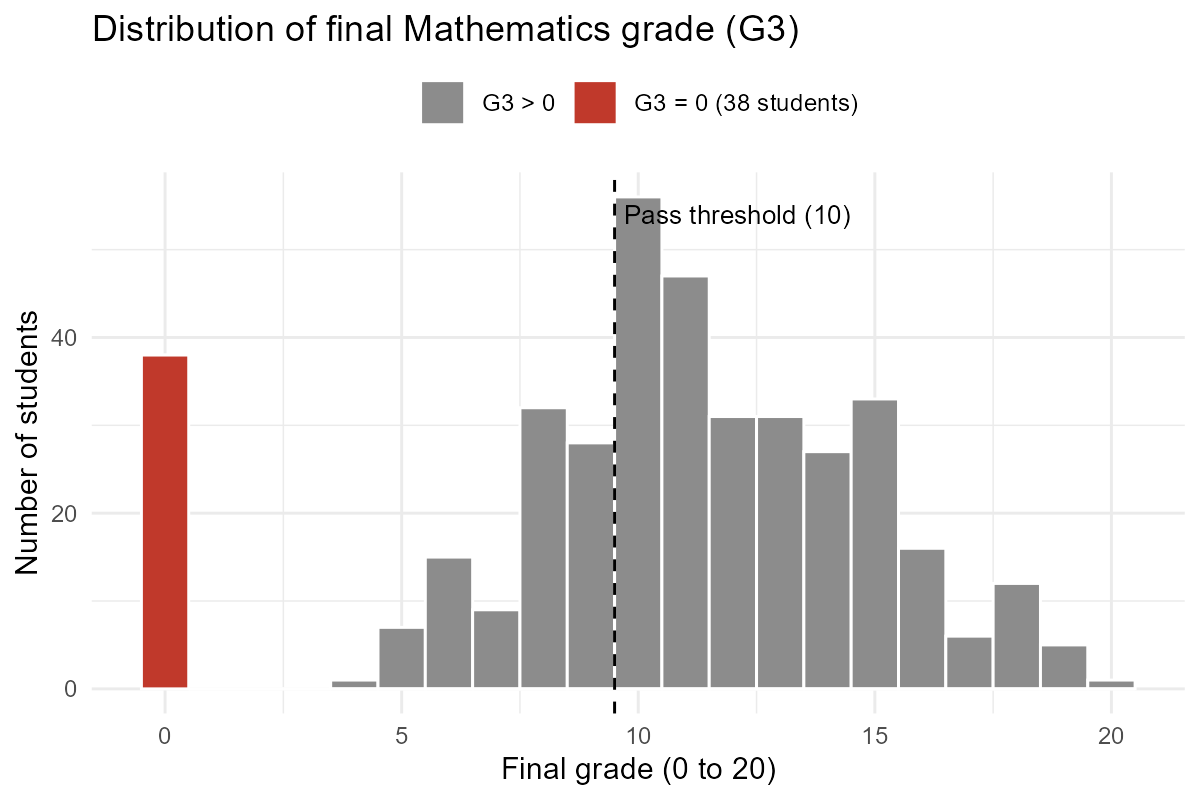
\includegraphics[width=0.60\textwidth]{fig1_g3_distribution.png}
\caption{Distribution of final mathematics grades, highlighting the cluster of 38 non-attendees at zero.}
\label{fig:dist}
\end{figure}

Performance differences across groups are substantial. Average grades drop progressively from 11.3 among students with clean academic records down to 8.1, 6.2, and 5.7 for those with one, two, or three-plus past failures (Figure~\ref{fig:groups}a). Socialising displays a slight non-linear trend: students who report going out very rarely score somewhat below average, those reporting low social outings peak at an average of 11.2, and those at the top end of the scale drop to 9.0 (Figure~\ref{fig:groups}b). Male students averaged slightly higher than female students (10.9 vs 10.0), with an associated pass rate of 70.6\% compared to 63.9\%.

\begin{figure}[H]
\centering
\begin{subfigure}{0.45\textwidth}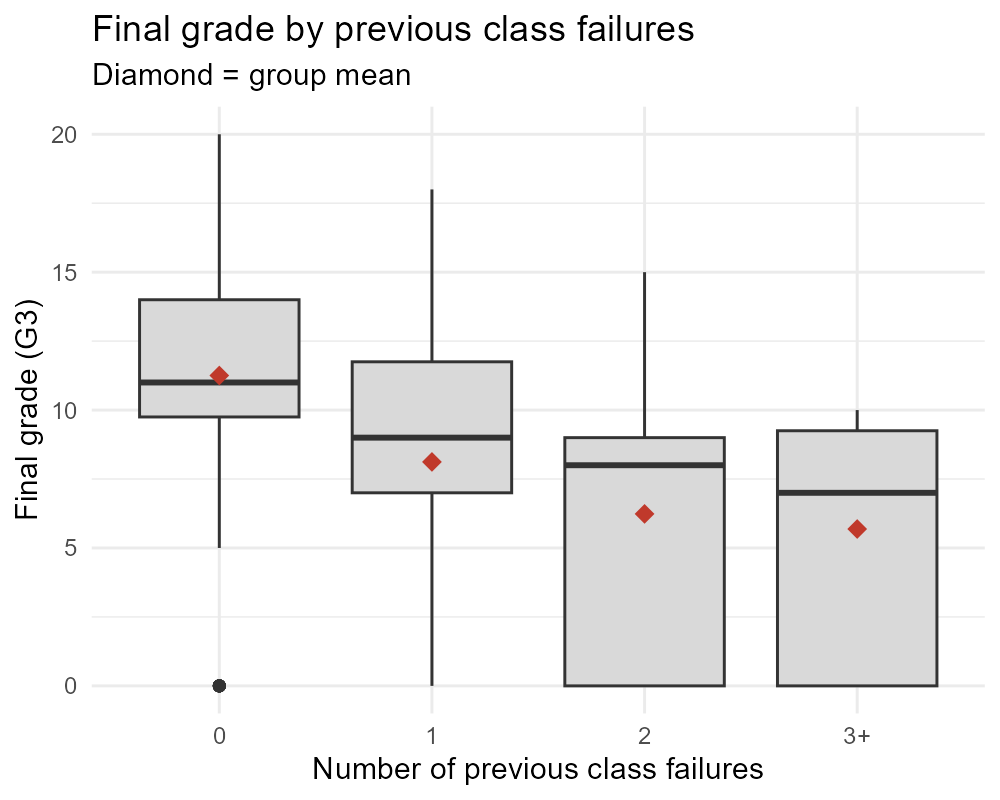
\includegraphics[width=\linewidth]{fig2_g3_by_failures.png}\caption{By previous failures}\end{subfigure}\hfill
\begin{subfigure}{0.45\textwidth}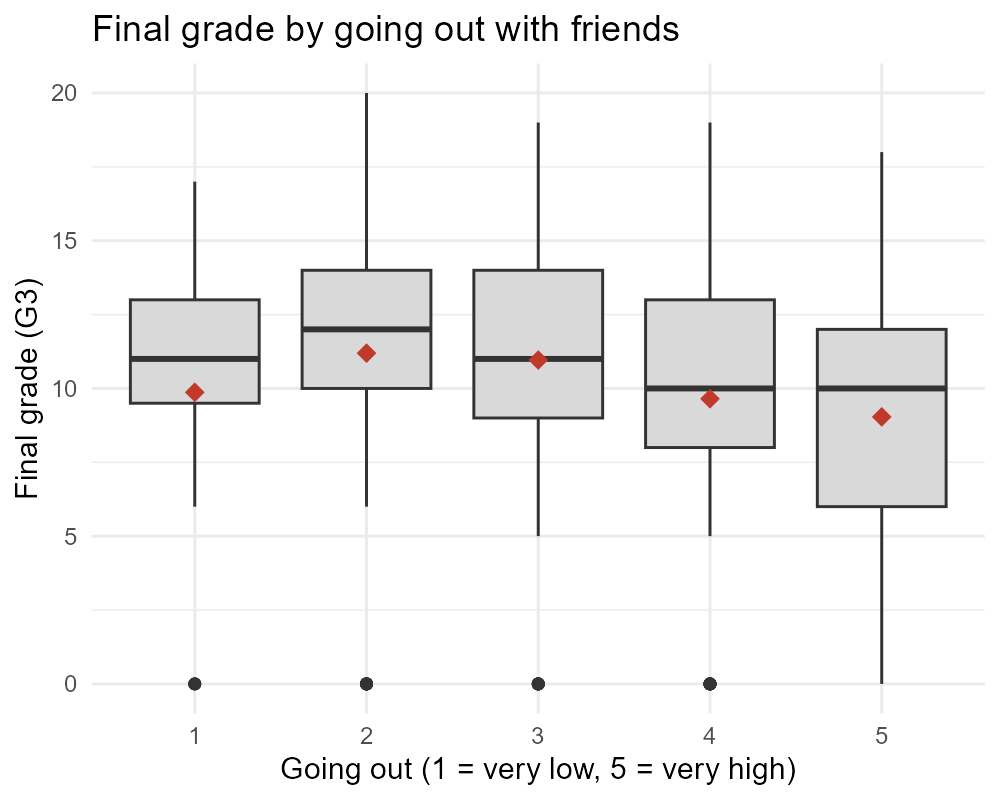
\includegraphics[width=\linewidth]{fig3_g3_by_goout.png}\caption{By going out frequency}\end{subfigure}
\caption{Grade distributions across key student characteristics (box: IQR, diamond: mean).}
\label{fig:groups}
\end{figure}

%==============================================================================
\section{Bivariate associations and variable choice}

Rank-order (Spearman) correlations largely mirrored Pearson coefficients across the ordinal indicators (full matrix in Appendix~A). Past failure count shows the clearest negative relationship with final score ($r = -0.36$), followed by maternal education ($r = 0.22$), age ($-0.16$), paternal education ($0.15$), and going out frequency ($-0.13$). Weekly study time correlates modestly ($r = 0.10$), while raw absences appear almost completely detached from grades overall ($r = 0.03$). Parental education levels are strongly collinear ($r = 0.62$), as are weekday and weekend drinking ($r = 0.65$); consequently, only one variable from each pair was considered for modelling to avoid redundancy.

\begin{figure}[H]
\centering
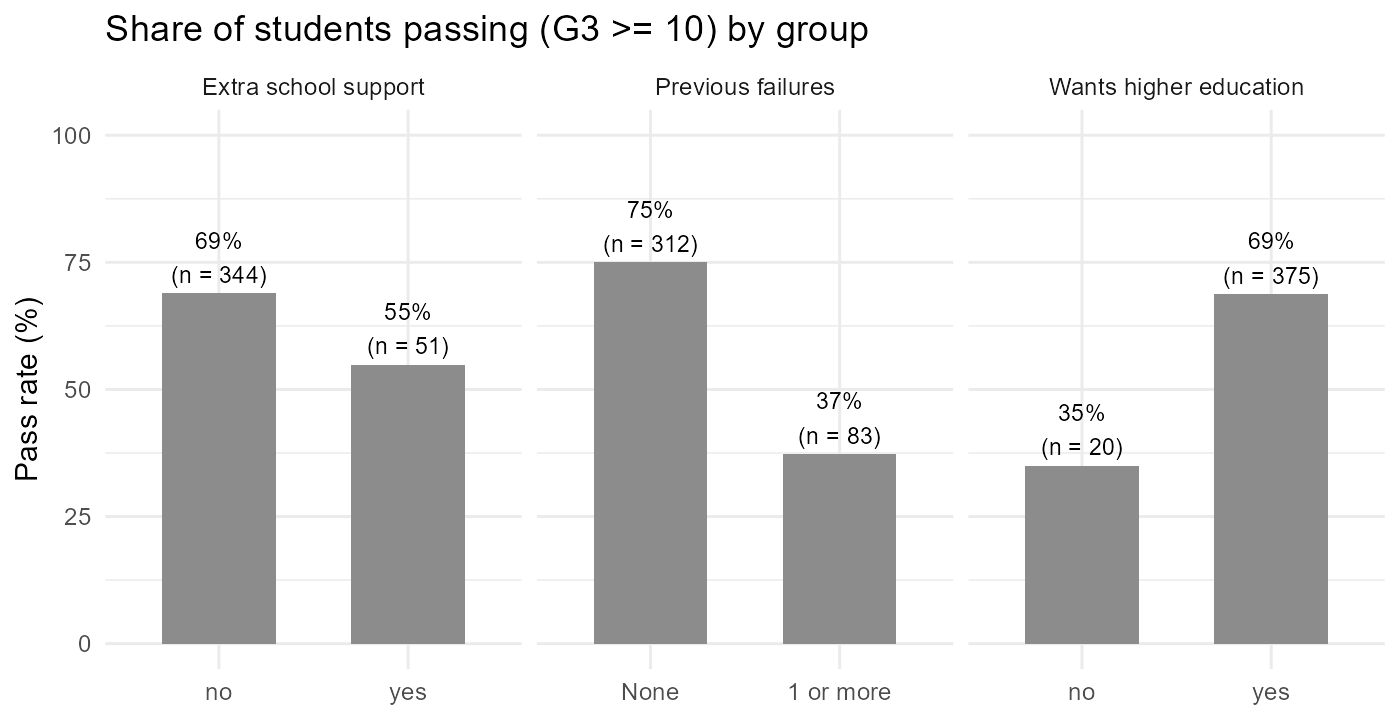
\includegraphics[width=0.74\textwidth]{fig5_pass_rates.png}
\caption{Pass rates ($\texttt{G3} \geq 10$) across selected binary indicators.}
\label{fig:pass}
\end{figure}

Group comparisons highlight similar divides. Students with prior failures pass at roughly half the rate of those without (37.3\% vs 75.0\%; $\chi^2 = 40, p < 0.001$). The pass rate among students not aiming for higher education is 35\% compared to 69\% for those who do ($p = 0.003$), though this group comprises only 20 individuals. Counterintuitively, students enrolled in remedial school support pass less often than those who are not (54.9\% vs 68.9\%, $p = 0.07$). This clearly reflects selection rather than an adverse effect of tutoring; support is allocated to students who are already struggling. For this reason, \texttt{schoolsup} was left out of the predictive regressions.

The apparent lack of relationship between absences and performance is driven by the 38 zero-grade students, all recorded with zero absences at the bottom-left of the scatter (Figure~\ref{fig:abs}). Once these 38 cases are removed, the trend between absences and grades turns negative, showing that the overall flat correlation is an artefact of data logging.

For the final models, I retained past failures, maternal education, going out, and sex as core background factors, and added study time, absences, and higher-education aspiration.

%==============================================================================
\section{Regression analysis}

The linear specification models \texttt{G3} against the seven selected variables, using female and no aspiration for higher education as reference levels (Table~\ref{tab:lin}).

\begin{table}[H]
\centering\small
\caption{Linear regression model for final Mathematics grade ($n = 395$).}
\label{tab:lin}
\begin{tabular}{lrrrr}
\toprule
Predictor & Estimate & 95\% CI & $t$ & $p$ \\
\midrule
Previous failures & $-1.80$ & $[-2.41,\ -1.20]$ & $-5.85$ & $<0.001$ \\
Mother's education & $0.49$ & $[0.09,\ 0.89]$ & $2.43$ & $0.016$ \\
Going out & $-0.46$ & $[-0.83,\ -0.08]$ & $-2.38$ & $0.018$ \\
Study time & $0.37$ & $[-0.15,\ 0.90]$ & $1.39$ & $0.164$ \\
Absences & $0.04$ & $[-0.02,\ 0.09]$ & $1.40$ & $0.162$ \\
Male & $1.41$ & $[0.52,\ 2.30]$ & $3.13$ & $0.002$ \\
Wants higher education & $1.78$ & $[-0.24,\ 3.80]$ & $1.73$ & $0.084$ \\
\midrule
\multicolumn{5}{l}{$R^2 = 0.186$, Adjusted $R^2 = 0.171$, Residual SD = 4.17 points.}\\
\bottomrule
\end{tabular}
\end{table}

Adjusting for other variables, every prior failure costs an estimated 1.8 points on the 20-point scale. A student with average profile values (secondary-educated mother, moderate social life, 2--5 hours study, 4 absences, female, aiming for university) has an expected score of 10.5 with no failures, dropping to 6.9 if she has repeated two years. Maternal education adds roughly half a point per level, while each step up the social outing scale reduces the expected mark by about half a point. Male students average 1.4 points higher when other predictors are held equal. Overall, the fit remains modest ($R^2 = 0.186$); more than four-fifths of grade variance remains uncaptured, and predictions carry an average uncertainty of over 4 marks.

\begin{table}[H]
\centering\small
\caption{Logistic regression model for passing final Mathematics ($n = 395$).}
\label{tab:log}
\begin{tabular}{lrrr}
\toprule
Predictor & Odds ratio & 95\% CI & $p$ \\
\midrule
Previous failures & $0.42$ & $[0.29,\ 0.59]$ & $<0.001$ \\
Mother's education & $1.11$ & $[0.89,\ 1.38]$ & $0.368$ \\
Going out & $0.71$ & $[0.57,\ 0.87]$ & $0.001$ \\
Study time & $1.09$ & $[0.81,\ 1.48]$ & $0.559$ \\
Absences & $0.98$ & $[0.96,\ 1.01]$ & $0.244$ \\
Male & $1.74$ & $[1.06,\ 2.89]$ & $0.030$ \\
Wants higher education & $2.13$ & $[0.71,\ 6.62]$ & $0.177$ \\
\bottomrule
\end{tabular}
\end{table}

The logistic model mirrors these patterns on the pass/fail margin (Table~\ref{tab:log}). Each past failure lowers the odds of passing by roughly 58\% ($\text{OR} = 0.42$), and each unit increase in going out reduces them by 29\% ($\text{OR} = 0.71$). Converted to probabilities for the baseline profile, a student with zero failures has a 72\% pass chance, which falls to 31\% with two past failures. Interestingly, maternal education shows no clear link to passing threshold itself ($p = 0.368$), despite its positive slope in the linear model. As a standalone classifier with a default 0.5 cut-off, the logistic model achieves 72.9\% overall accuracy, which is only slightly above the naive baseline of predicting a pass for everyone (67.1\%), successfully flagging only 35\% of actual course failures.

%==============================================================================
\section{Diagnostics and sensitivity analysis}

Residual plots from the linear fit reveal a distinct structural problem: the 38 zero-grade records line up in a clean diagonal trace well below the main scatter (Figure~\ref{fig:resid}a). Beyond this subgroup, residuals remain reasonably balanced around zero, aside from some boundary compression at the low end. The Q-Q plot (Appendix~A) confirms this substantial left-tail distortion. Multicollinearity is negligible, with variance inflation factors between 1.03 and 1.19.

\begin{figure}[H]
\centering
\begin{subfigure}{0.46\textwidth}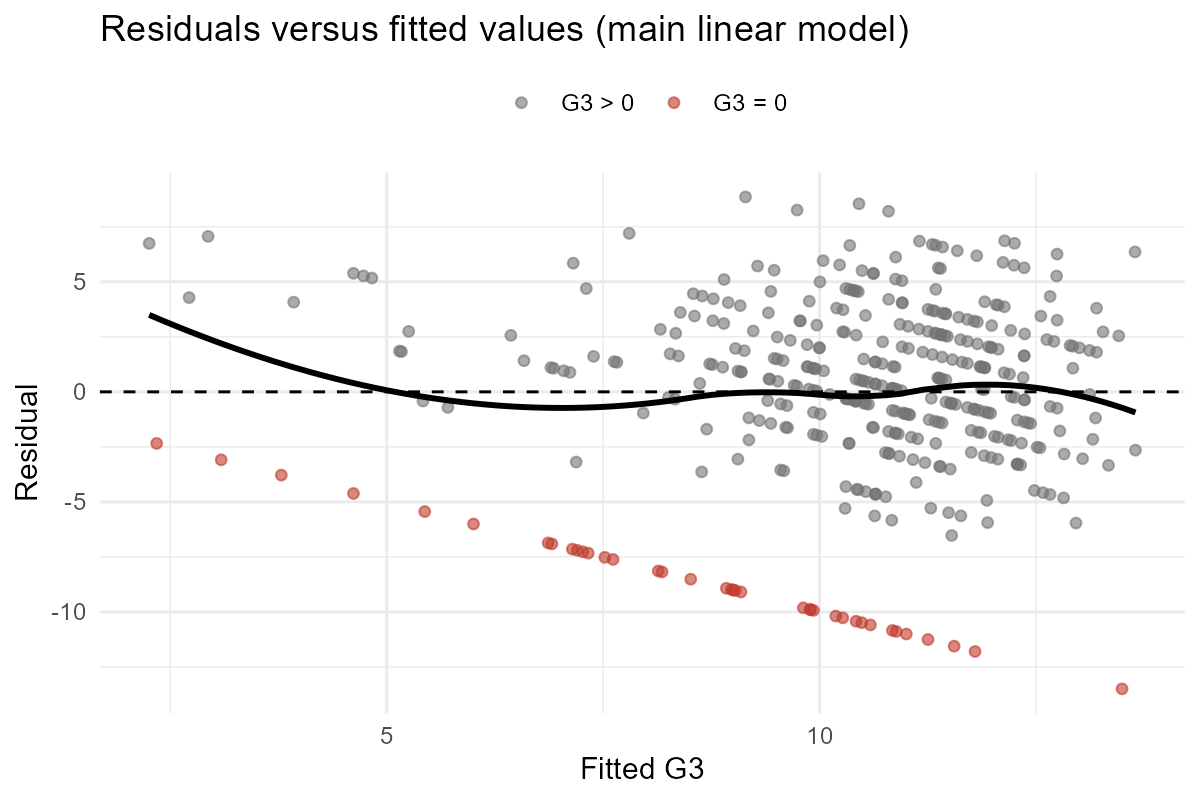
\includegraphics[width=\linewidth]{fig8_residuals_vs_fitted.png}\caption{Residuals vs fitted values}\end{subfigure}\hfill
\begin{subfigure}{0.46\textwidth}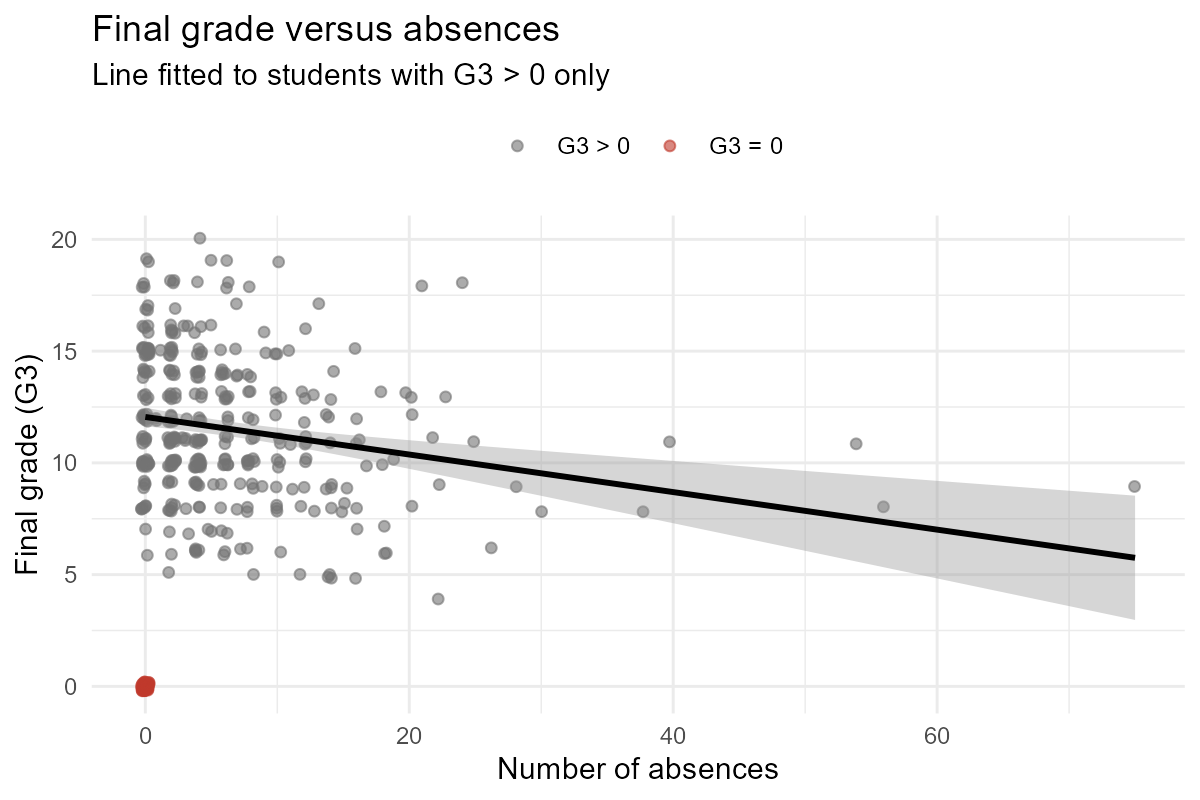
\includegraphics[width=\linewidth]{fig6_absences_vs_g3.png}\caption{Absences vs final grade}\label{fig:abs}\end{subfigure}
\caption{Residual behaviour and the impact of the non-attending cohort (marked red).}
\label{fig:resid}
\end{figure}

Excluding these 38 cases in a sensitivity run substantively alters several parameters (Appendix~C). Most strikingly, the coefficient for absences flips from slightly positive to clearly negative ($-0.07$ points per day missed, $p < 0.001$). The penalty associated with past failures is cut roughly in half (from $-1.80$ to $-0.98$), reflecting that non-completers carried a disproportionate record of prior failures (0.92 vs 0.27 on average). Study time turns marginally significant ($p = 0.04$), while the higher-education coefficient collapses and the male advantage weakens. Meanwhile, the estimated effects for maternal education and going out remain virtually identical, demonstrating that their associations do not depend on how dropouts are handled.

%==============================================================================
\section{Discussion and limitations}

Because these data reflect an observational snapshot of two public secondary schools in 2005--2006, the associations cannot be interpreted causally. One cannot conclude that simply limiting a student's social life would directly produce higher test scores. 

Unobserved factors are likely doing much of the explanatory work. Prior foundational math competence, individual drive, household income, teacher effectiveness, and peer dynamics were not tracked. Past failures are most likely an indicator of cumulative academic struggle rather than an independent causal mechanism. Similarly, self-reported measures on brief integer scales carry unavoidable noise and reporting bias. 

In summary, past academic difficulty remains the most reliable warning sign for poor final performance in this dataset, with family background and social balance playing secondary, consistent roles. However, the data leave over 80\% of student achievement unexplained, and several baseline conclusions—notably the role of absences—are heavily skewed by how non-attending students are handled. The model provides a broad overview of risk factors across groups, but it lacks the precision needed to guide individual interventions.

\vspace{1ex}
\noindent\textbf{References}\\[0.3ex]
{\small
Cortez, P. (2008). \emph{Student Performance} [Dataset]. UCI Machine Learning Repository. \url{https://doi.org/10.24432/C5TG7T}\\
Cortez, P., \& Silva, A. (2008). Using data mining to predict secondary school student performance. In \emph{Proceedings of the 5th Future Business Technology Conference (FUBUTEC 2008)}, 5--12.\\
R Core Team (2023). \emph{R: A language and environment for statistical computing} (version 4.3.3). Packages: ggplot2, dplyr, broom.
}

%==============================================================================
\clearpage
\appendix
\section*{Appendix A. Correlation heatmap and Q-Q plot}
\begin{figure}[H]
\centering
\begin{subfigure}{0.54\textwidth}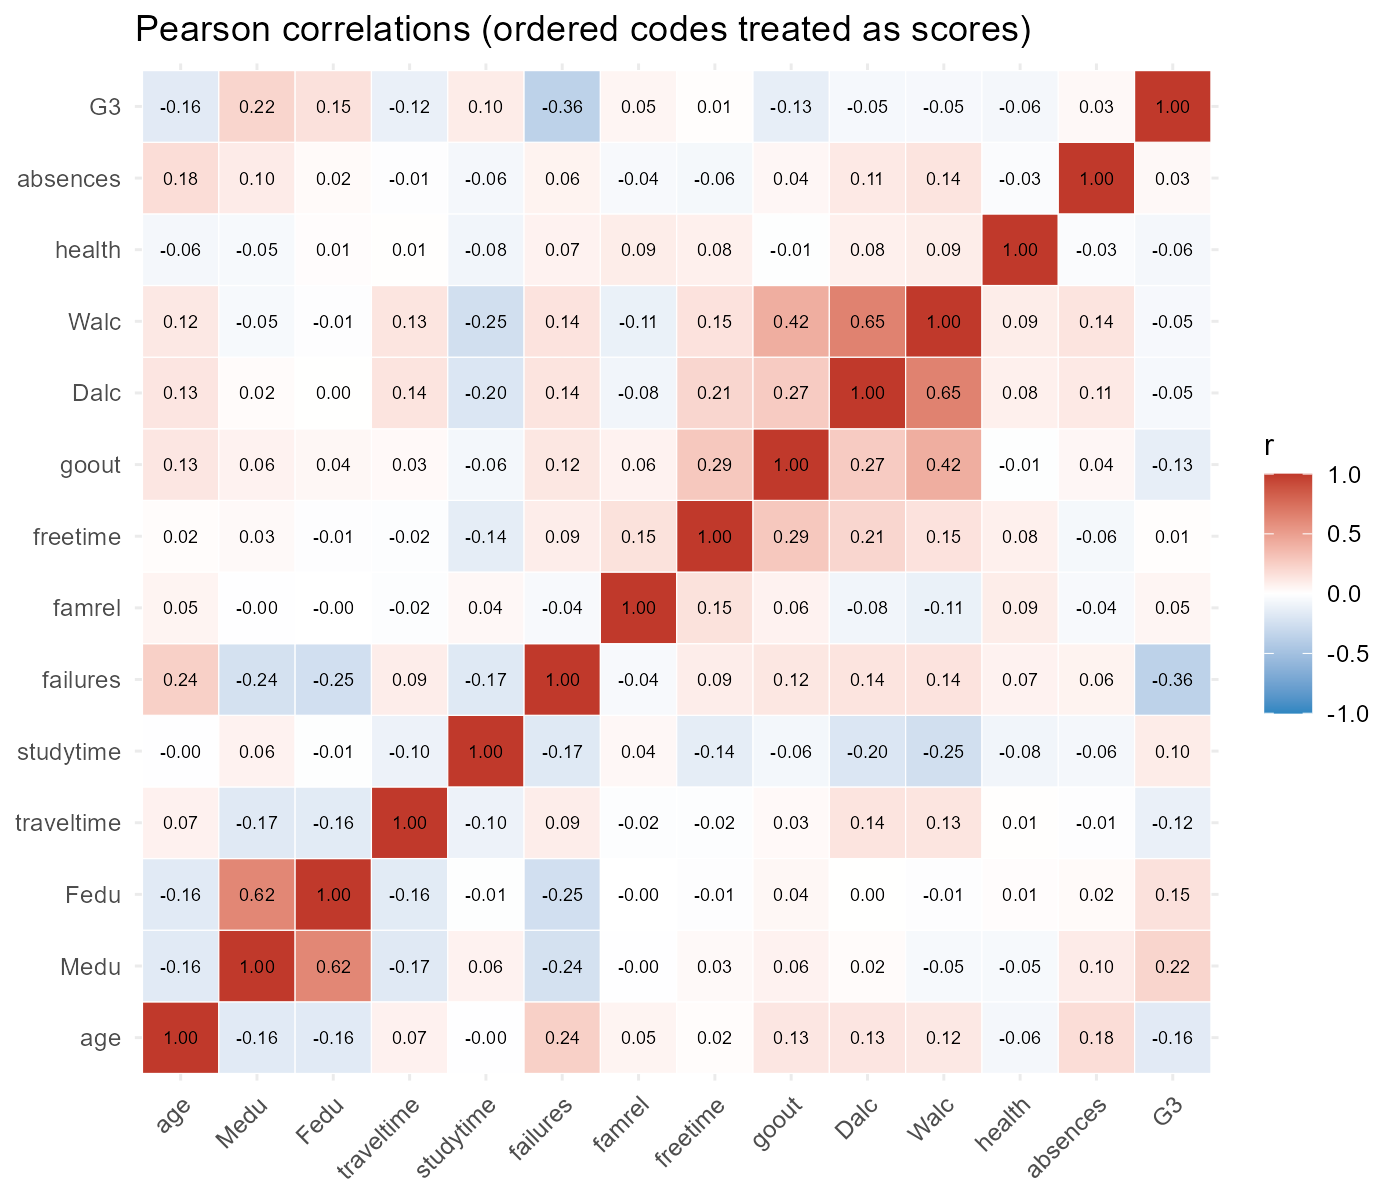
\includegraphics[width=\linewidth]{fig4_correlation_heatmap.png}\end{subfigure}\hfill
\begin{subfigure}{0.42\textwidth}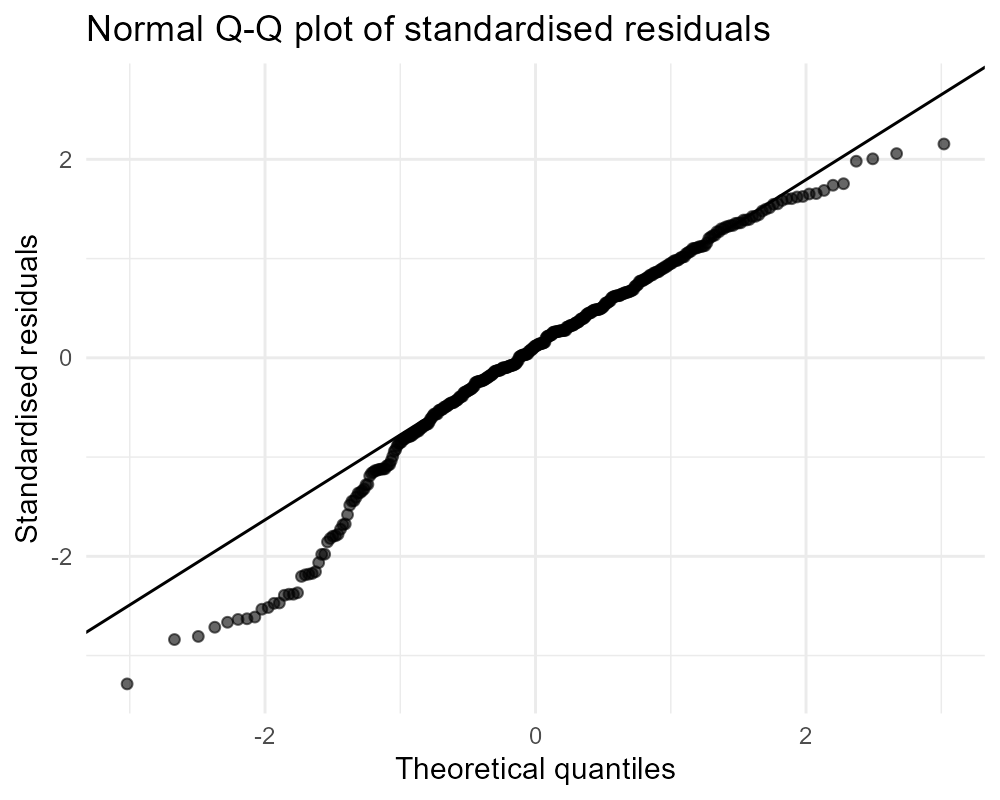
\includegraphics[width=\linewidth]{figA_qq_plot.png}\end{subfigure}
\caption{Left: Correlation matrix. Right: Normal Q-Q plot of standardised residuals from the full linear fit.}
\end{figure}

\section*{Appendix B. Logistic model predictions}
\begin{figure}[H]
\centering
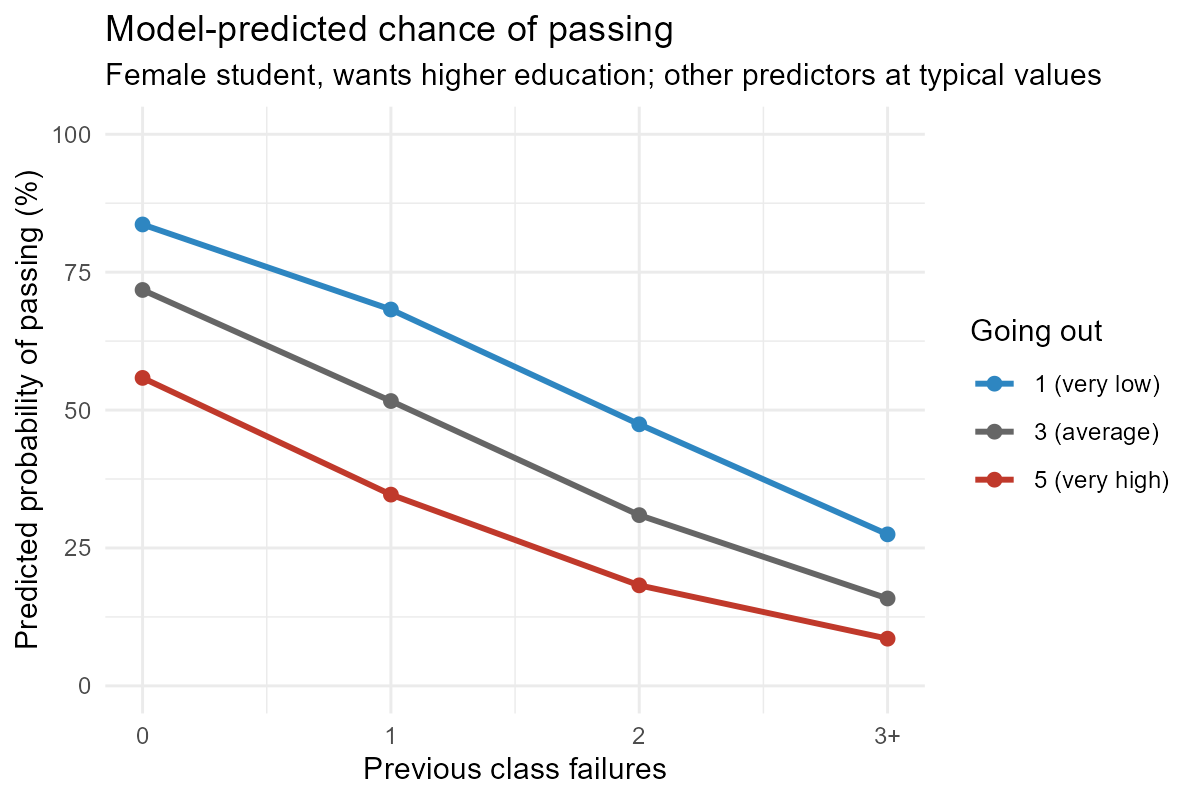
\includegraphics[width=0.58\textwidth]{fig7_predicted_pass_probability.png}
\caption{Predicted pass probabilities across past failures and social outings for a female student aspiring to higher education.}
\end{figure}

\section*{Appendix C. Sensitivity analysis: complete cases vs excluding G3 = 0}
\begin{table}[H]
\centering\small
\begin{tabular}{lrrrr}
\toprule
 & \multicolumn{2}{c}{Linear: coefficient [95\% CI]} & \multicolumn{2}{c}{Logistic: odds ratio [95\% CI]} \\
\cmidrule(lr){2-3}\cmidrule(lr){4-5}
Predictor & All ($n=395$) & $G3 > 0$ ($n=357$) & All ($n=395$) & $G3 > 0$ ($n=357$) \\
\midrule
Failures & $-1.80$ $[-2.41, -1.20]$ & $-0.98$ $[-1.47, -0.48]$ & 0.42 [0.29, 0.59] & 0.51 [0.35, 0.74] \\
Mother's educ. & $0.49$ $[0.09, 0.89]$ & $0.46$ $[0.17, 0.76]$ & 1.11 [0.89, 1.38] & 1.10 [0.85, 1.42] \\
Going out & $-0.46$ $[-0.83, -0.08]$ & $-0.46$ $[-0.75, -0.18]$ & 0.71 [0.57, 0.87] & 0.65 [0.51, 0.83] \\
Study time & $0.37$ $[-0.15, 0.90]$ & $0.42$ $[0.02, 0.81]$ & 1.09 [0.81, 1.48] & 1.13 [0.80, 1.60] \\
Absences & $0.04$ $[-0.02, 0.09]$ & $-0.07$ $[-0.10, -0.03]$ & 0.98 [0.96, 1.01] & 0.95 [0.92, 0.98] \\
Male & $1.41$ $[0.52, 2.30]$ & $0.81$ $[0.16, 1.47]$ & 1.74 [1.06, 2.89] & 1.49 [0.86, 2.63] \\
Wants higher ed. & $1.78$ $[-0.24, 3.80]$ & $0.09$ $[-1.60, 1.79]$ & 2.13 [0.71, 6.62] & 1.40 [0.38, 5.02] \\
\midrule
$R^2$ (linear) & 0.186 & 0.180 & & \\
\bottomrule
\end{tabular}
\end{table}

\end{document}